% Chinese translation assembled from source/blocks.json.

% See source/translation.py for the translation and source/build_tex.py for assembly.

% source-block: 271211a5-58b7-8046-af48-c3129693f3f1 (header; source-index: 52)

\hypertarget{src-271211a5-58b7-8046-af48-c3129693f3f1}{}
\section*{3. 剖析训练崩溃}
\phantomsection
\addcontentsline{toc}{section}{3. 剖析训练崩溃}


% source-block: 271211a5-58b7-80f8-b824-f71b5fe11763 (sub_header; source-index: 53)

\hypertarget{src-271211a5-58b7-80f8-b824-f71b5fe11763}{}
\subsection*{3.0 实验设置}
\phantomsection
\addcontentsline{toc}{subsection}{3.0 实验设置}


% source-block: 271211a5-58b7-8011-872c-ff8c4e24455f (text; source-index: 54)

除非另有说明，第 3 节和第 4 节的实验均在 \href{https://github.com/search?q=verl&type=repositories}{VeRL} 框架下采用 TIR 设置进行，使用 vLLM v1 采样器（AsyncvLLMServer）、Qwen3-14B-Base 模型和 GRPO 算法，并在 L20 GPU 集群上运行。


% source-block: 277211a5-58b7-80de-809d-ed58cc96a034 (divider; source-index: 55)

% source-block: 271211a5-58b7-8057-8bd8-da62a18d6e3a (sub_header; source-index: 56)

\hypertarget{src-271211a5-58b7-8057-8bd8-da62a18d6e3a}{}
\subsection*{3.1 度量不匹配：\texttt{vllm-kl} 指标}
\phantomsection
\addcontentsline{toc}{subsection}{3.1 度量不匹配：vllm-kl 指标}


% source-block: 271211a5-58b7-80be-bf0e-d70767335f76 (text; source-index: 57)

一种直接衡量训练与推理不匹配的指标是 \code{vllm-kl}：


% source-block: 271211a5-58b7-80f6-9ba6-e24d819d0485 (equation; source-index: 58)


\[
\adjustbox{max width=0.98\linewidth}{$\displaystyle \mathbb{E}_{s\sim d_{\textcolor{red}{\pi^{\text{vllm}}_\theta}}}\left[\text{KL}\left(\textcolor{red}{\pi^{\text{vllm}}_\theta}\left(\cdot|s\right),\textcolor{blue}{\pi^{\text{fsdp}}_\theta}\left(\cdot|s\right)\right)\right]$}
\]

\vspace{-1em}

\[
\adjustbox{max width=0.98\linewidth}{$\displaystyle {}= \mathbb{E}_{s\sim d_{\textcolor{red}{\pi^{\text{vllm}}_\theta}},a\sim {\textcolor{red}{\pi^{\text{vllm}}_\theta}\left(\cdot|s\right)}} \left[\log\left(\frac{\textcolor{red}{\pi^{\text{vllm}}_\theta}(a|s)}{\textcolor{blue}{\pi^{\text{fsdp}}_\theta}(a|s)}\right)\right],$}
\]


% source-block: 271211a5-58b7-80c4-a955-ea90e314216d (text; source-index: 59)

其中，$d_\pi$ 是策略 $\pi$ 的状态占用测度，$s$ 是上下文前缀（状态），$a$ 是词元（动作）。我们的实验涉及工具调用，因此响应 $y$ 可能包含工具返回内容；\code{vllm-kl} 指标只统计模型自身生成的词元。假设已能取得推理引擎的词元概率，下面的代码给出了在 \href{https://github.com/search?q=verl&type=repositories}{VeRL} 中使用 \href{http://joschu.net/blog/kl-approx.html}{K3 估计器}计算该指标的实现。


% source-block: 271211a5-58b7-804d-a515-cf72e195691b (toggle; source-index: 60)

\hypertarget{src-271211a5-58b7-804d-a515-cf72e195691b}{}
\paragraph*{\texttt{vllm-kl} 的 K3 估计器代码（展开原文折叠内容）}


% source-block: 271211a5-58b7-8012-a9f1-e15e76434fd9 (code; source-index: 61)

\lstinputlisting{source/k3_vllm_kl.py}

% source-block: 277211a5-58b7-80e1-92cf-f20011be2769 (divider; source-index: 62)

% source-block: 271211a5-58b7-806f-a251-c6e6bcade90c (sub_header; source-index: 63)

\hypertarget{src-271211a5-58b7-806f-a251-c6e6bcade90c}{}
\subsection*{3.2 预警信号：相互关联的不稳定性}
\phantomsection
\addcontentsline{toc}{subsection}{3.2 预警信号：相互关联的不稳定性}


% source-block: 271211a5-58b7-8043-b721-efdbf1c851cb (text; source-index: 64)

第一个线索是：高 \code{vllm-kl} 值并非孤立事件，而是与其他不稳定迹象高度相关。


% source-block: 271211a5-58b7-80e6-a27d-df95d40e31e0 (sub_sub_header; source-index: 65)

\hypertarget{src-271211a5-58b7-80e6-a27d-df95d40e31e0}{}
\subsubsection*{3.2.1 FSDP 熵与奖励的波动}


% source-block: 271211a5-58b7-808f-a90f-df4730390799 (text; source-index: 66)

在许多实验中，我们观察到 \code{vllm-kl} 的异常尖峰通常会同时伴随 FSDP 策略 $\pif$ 的熵与奖励的异常波动。图 2 给出了直观例子：熵尖峰与 \code{vllm-kl} 尖峰的位置几乎完全对应。奖励没有表现出同样明显的相关性，但在约第 250 步处，巨大的 \code{vllm-kl} 尖峰触发了一个低质量批次的生成，奖励也随之明显下跌。这意味着当不匹配较大时，vLLM 策略 $\piv$ 与 FSDP 策略 $\pif$ 都进入了不稳定区域。


% source-block: 271211a5-58b7-8055-8f35-c4a618ee5fed (image; source-index: 67)

\begin{figure}[H]
\centering
% source-block: 271211a5-58b7-8055-8f35-c4a618ee5fed (image)
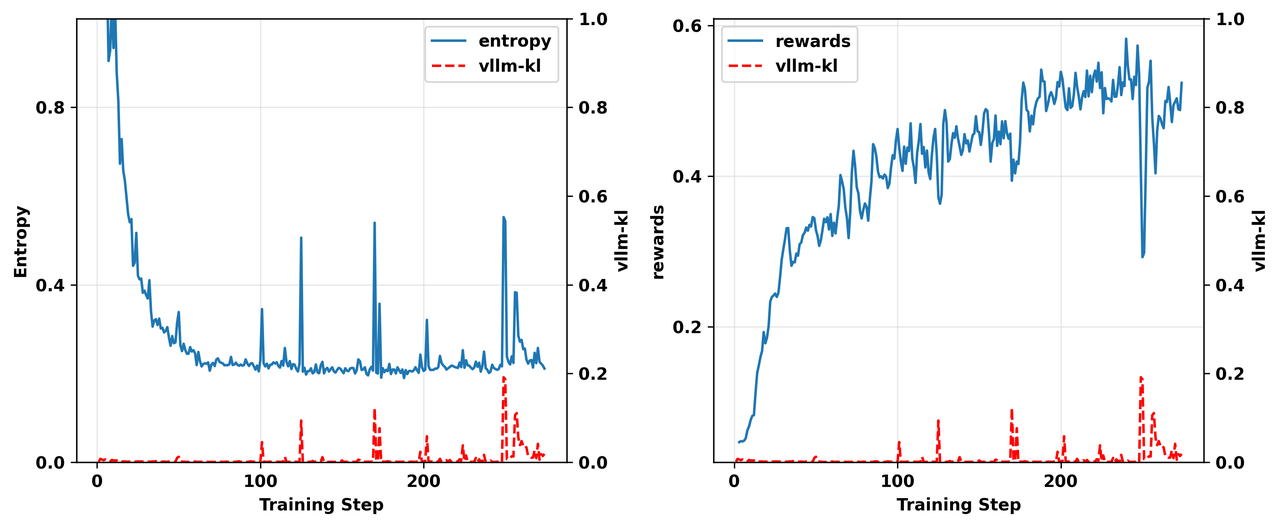
\includegraphics[width=\linewidth,height=0.64\textheight,keepaspectratio]{figures/image-02.png}
\caption*{\textbf{图 2。}同策略实验的熵（左）、奖励（右）与 \code{vllm-kl} 的对照，展示训练期间它们之间的相关性。}
\end{figure}


% source-block: 277211a5-58b7-805f-b028-ed2aaa0553fc (divider; source-index: 68)

% source-block: 271211a5-58b7-80b3-b8f8-eb93ea995636 (sub_sub_header; source-index: 69)

\hypertarget{src-271211a5-58b7-80b3-b8f8-eb93ea995636}{}
\subsubsection*{3.2.2 FSDP 困惑度和梯度范数上升，最终导致策略崩溃}


% source-block: 271211a5-58b7-8048-9746-ef5351a74003 (text; source-index: 70)

更关键的是，我们观察到 \code{vllm-kl} 的尖峰会同时伴随 \code{fsdp-ppl} 指标和梯度范数的爆炸。在实验中，响应 $y$ 的 FSDP \href{https://www.wikiwand.com/en/articles/Perplexity}{困惑度（PPL）}计算如下：


% source-block: 271211a5-58b7-8054-8737-dd5a1b74c83c (equation; source-index: 71)


\[
\adjustbox{max width=0.98\linewidth}{$\displaystyle \text{fsdp-ppl}:  \exp\left(\frac{-1}{\left| \mathcal{T} _{\mathcal{M}}\left( y \right) \right|}\sum_{t\in \mathcal{T} _{\mathcal{M}}\left( y \right)}{\log \textcolor{blue}{\pi _{\theta}^{\text{fsdp}}}\left( y_t|y_{<t} \right)}\right)$}
\]


% source-block: 271211a5-58b7-80a7-bc39-d63c27611086 (text; source-index: 72)

其中，$\mathcal T_{\mathcal M}(y)$ 是响应 $y$ 中由模型自身生成的词元索引集合。最终的 \code{fsdp-ppl} 指标，是一个批次中所有响应的困惑度的平均值。图 3 展示了同策略与异策略两种 GRPO 实验结果。两次实验中，\code{vllm-kl} 的尖峰几乎都精确对应着 \code{fsdp-ppl} 和梯度范数的爆炸。此外，训练奖励崩溃之前，\code{vllm-kl} 已经明显上升。


% source-block: 271211a5-58b7-8012-87d3-ce3f15ed3061 (image; source-index: 73)

\begin{figure}[H]
\centering
% source-block: 271211a5-58b7-8012-87d3-ce3f15ed3061 (image)
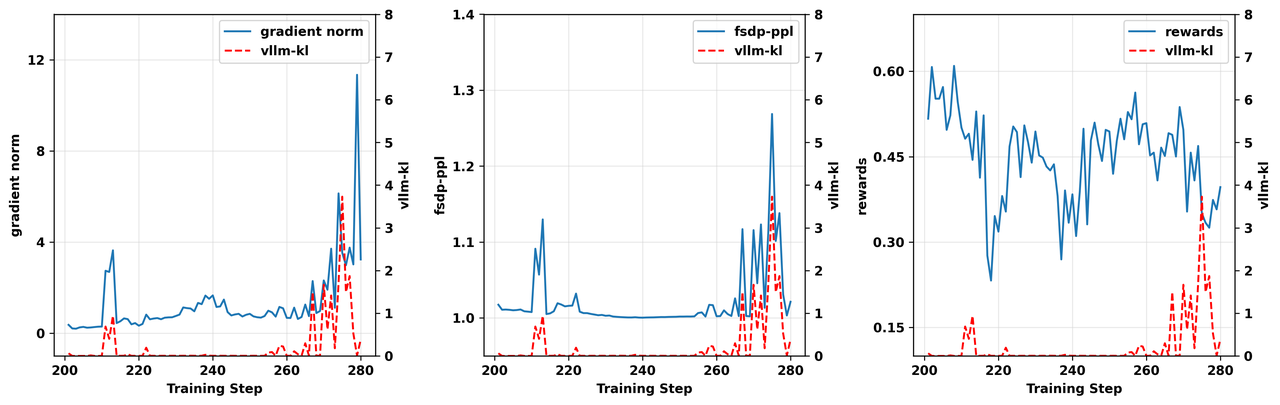
\includegraphics[width=\linewidth,height=0.64\textheight,keepaspectratio]{figures/image-03.png}
\par\smallskip
% source-block: 271211a5-58b7-8046-aba6-f54c74a49cf2 (image)
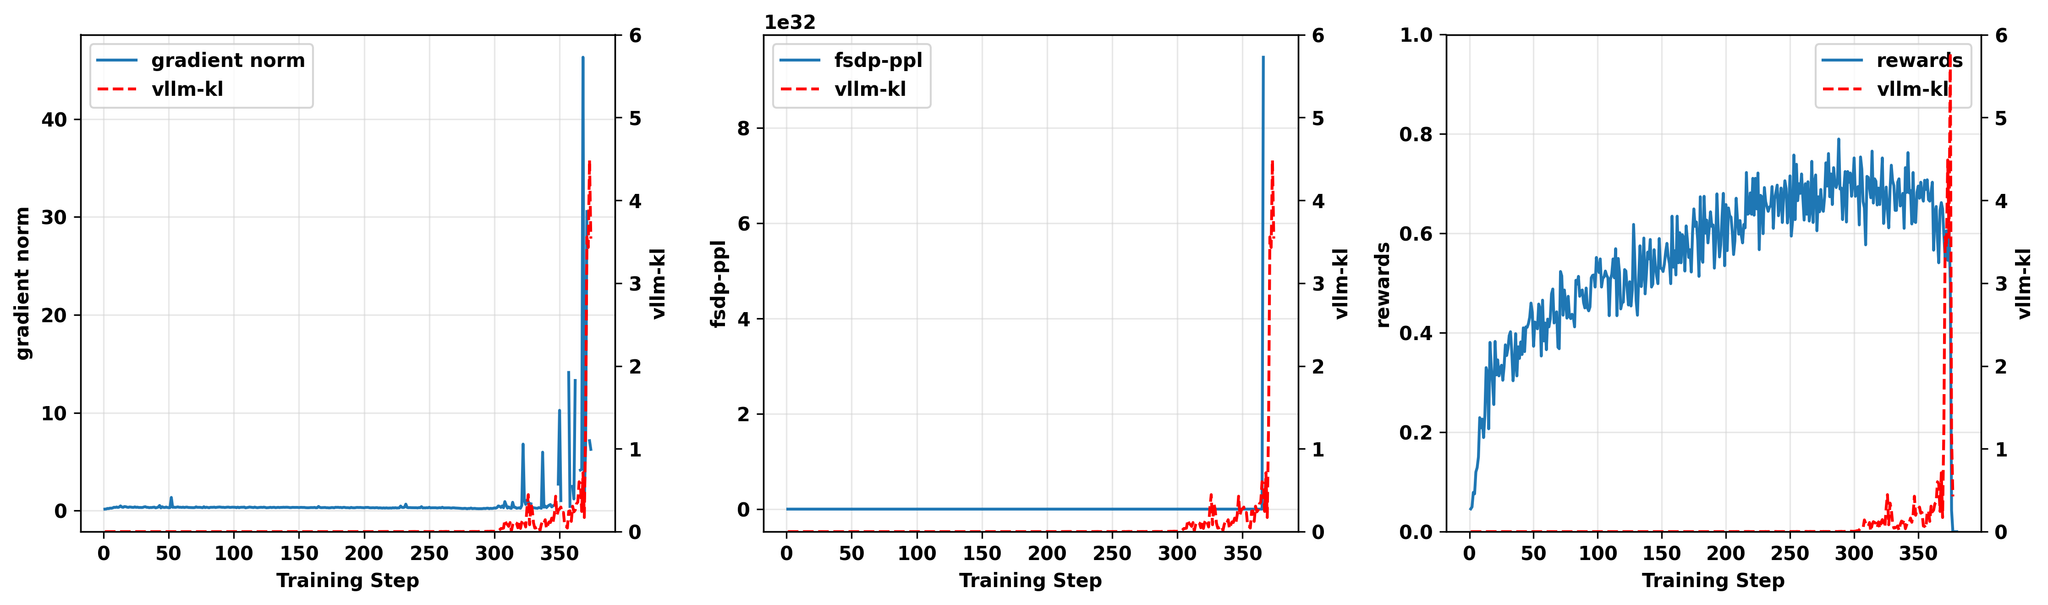
\includegraphics[width=\linewidth,height=0.64\textheight,keepaspectratio]{figures/image-04.png}
\par\smallskip
\caption*{\textbf{图 3。}同策略实验第 200--280 步的结果（上），以及 \code{clip-higher=0.28} 的异策略实验结果（下）。梯度范数（左）、\code{fsdp-ppl}（中）、奖励（右）分别与 \code{vllm-kl} 对照，展示训练期间的相关性。}
\end{figure}


% source-block: 271211a5-58b7-8046-aba6-f54c74a49cf2 (image; source-index: 74)

% source-block: 271211a5-58b7-80f1-b8fd-fd93435d5365 (text; source-index: 75)

在我们的实验中，模型自身生成的序列至少包含几百个词元，因此作者认为，在训练后期 PPL 维持在 1 附近更为合理。然而，在训练与推理不匹配显著、即 \code{vllm-kl} 很高的批次中，\code{fsdp-ppl} 出现了爆炸。这表明，FSDP 引擎为推理策略采样得到的词元分配了灾难性低的概率，从而导致梯度爆炸。这一观察帮助我们进一步定位不匹配更容易发生的位置。后文将看到：这些 FSDP 概率极低的词元在被采样时，其 vLLM 概率远没有这么低。


% source-block: 277211a5-58b7-8053-933b-eb574993d0ce (divider; source-index: 76)

% source-block: 271211a5-58b7-8043-9a6b-f4222291f060 (sub_header; source-index: 77)

\hypertarget{src-271211a5-58b7-8043-9a6b-f4222291f060}{}
\subsection*{3.3 关键证据：低概率词元陷阱}
\phantomsection
\addcontentsline{toc}{subsection}{3.3 关键证据：低概率词元陷阱}


% source-block: 277211a5-58b7-8056-afbf-fa0d227e8459 (text; source-index: 78)

\textbf{不匹配并非均匀发生。}


% source-block: 277211a5-58b7-804c-b071-d15a4d40365e (text; source-index: 79)

通过分析 \code{vllm-kl} 水平不同的批次，我们发现了鲜明的模式：\textbf{对 vLLM 推理引擎而言概率较低的词元，其偏差最为严重。}当词元的推理概率趋近于零时，训练概率可能进一步低上多个数量级，导致 PPL 和梯度趋于无穷。为尽量提高结论的普适性，我们从不同实验、不同训练步中，选取了崩溃之前采样的批次。这些批次均具有相对较高的 \code{vllm-kl}，便于在现象明显的条件下研究不匹配模式。我们按以下三个区间收集 rollout 批次，每组包含五个批次，约 500 万个词元：


% source-block: 271211a5-58b7-8010-8a35-e7633703fd9b (bulleted_list; source-index: 80)

\begin{itemize}

\item \textbf{第 1 组（低）：}每个 rollout 批次的 \code{vllm-kl} 不大于 $10^{-3}$，使用 H20 GPU 采样。

% source-block: 271211a5-58b7-8015-93c9-e4e2ef8301f1 (bulleted_list; source-index: 81)

\item \textbf{第 2 组（中）：}每个 rollout 批次的 \code{vllm-kl} 位于 $[10^{-3},2\times10^{-2}]$，使用 L20 GPU 采样。

% source-block: 271211a5-58b7-800a-88cd-e2fe0fb1c394 (bulleted_list; source-index: 82)

\item \textbf{第 3 组（高）：}每个 rollout 批次的 \code{vllm-kl} 位于 $[2\times10^{-2},10^{-1}]$，使用 L20 GPU 采样。

\end{itemize}

% source-block: 271211a5-58b7-80dd-83a4-c319ae9b7b6d (text; source-index: 83)

图 4(a)、4(b)、4(c) 展示了不同 \code{vllm-kl} 量级下，vLLM 输出概率 $\piv(a\mid s)$ 与不匹配程度 $\log\pif(a\mid s)-\log\piv(a\mid s)$ 之间的关系。


% source-block: 271211a5-58b7-8025-976d-c69c3de0ef2d (image; source-index: 84)

\begin{figure}[H]
\centering
% source-block: 271211a5-58b7-8025-976d-c69c3de0ef2d (image)
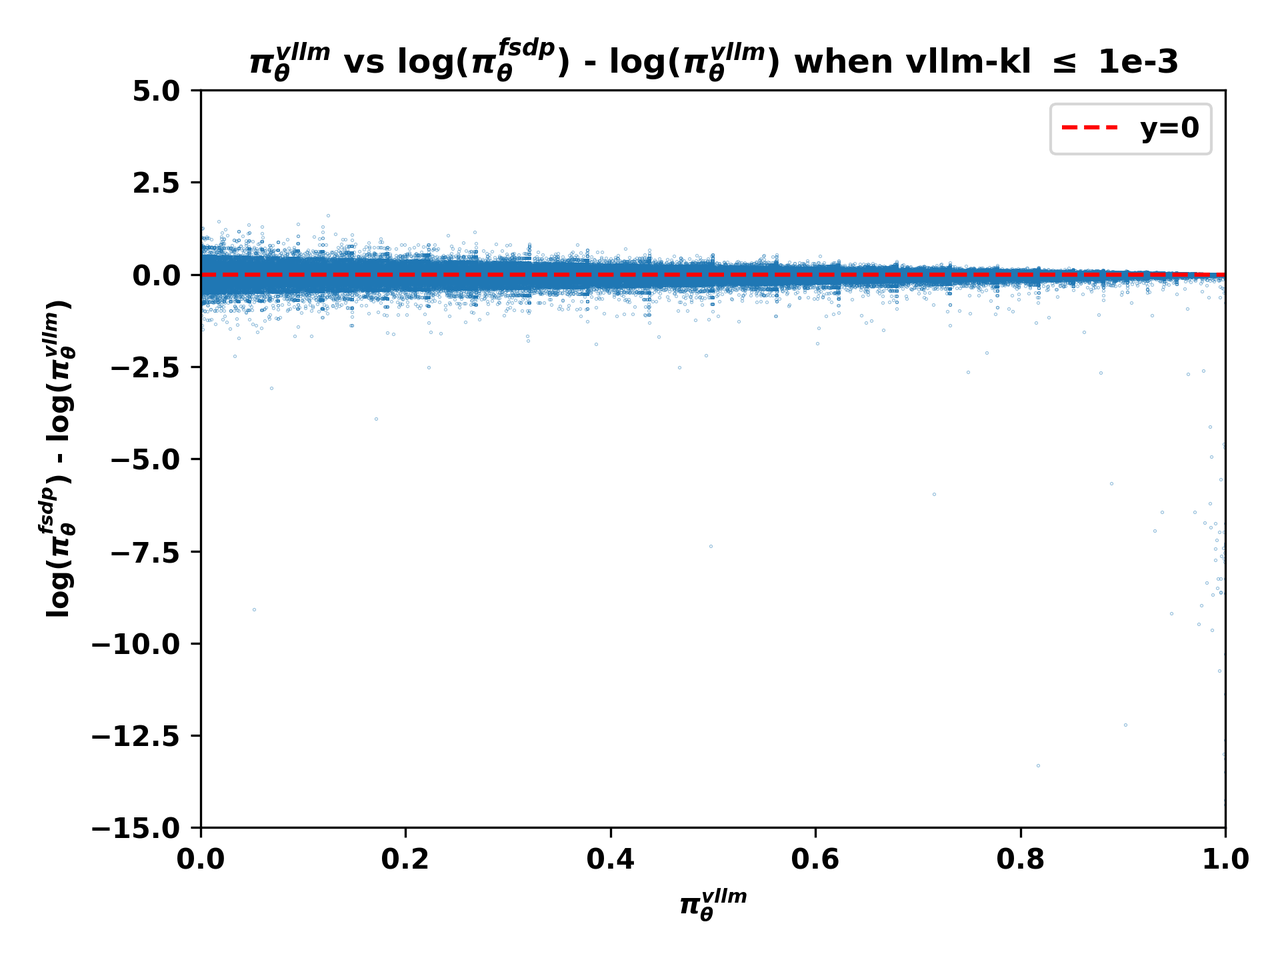
\includegraphics[width=\linewidth,height=0.64\textheight,keepaspectratio]{figures/image-05.png}
\caption*{\textbf{图 4(a)。}第 1 组批次中，词元的 $\piv$ 与 $\log\pif-\log\piv$ 的关系。}
\end{figure}


% source-block: 271211a5-58b7-8084-87e0-d30121785272 (image; source-index: 85)

\begin{figure}[H]
\centering
% source-block: 271211a5-58b7-8084-87e0-d30121785272 (image)
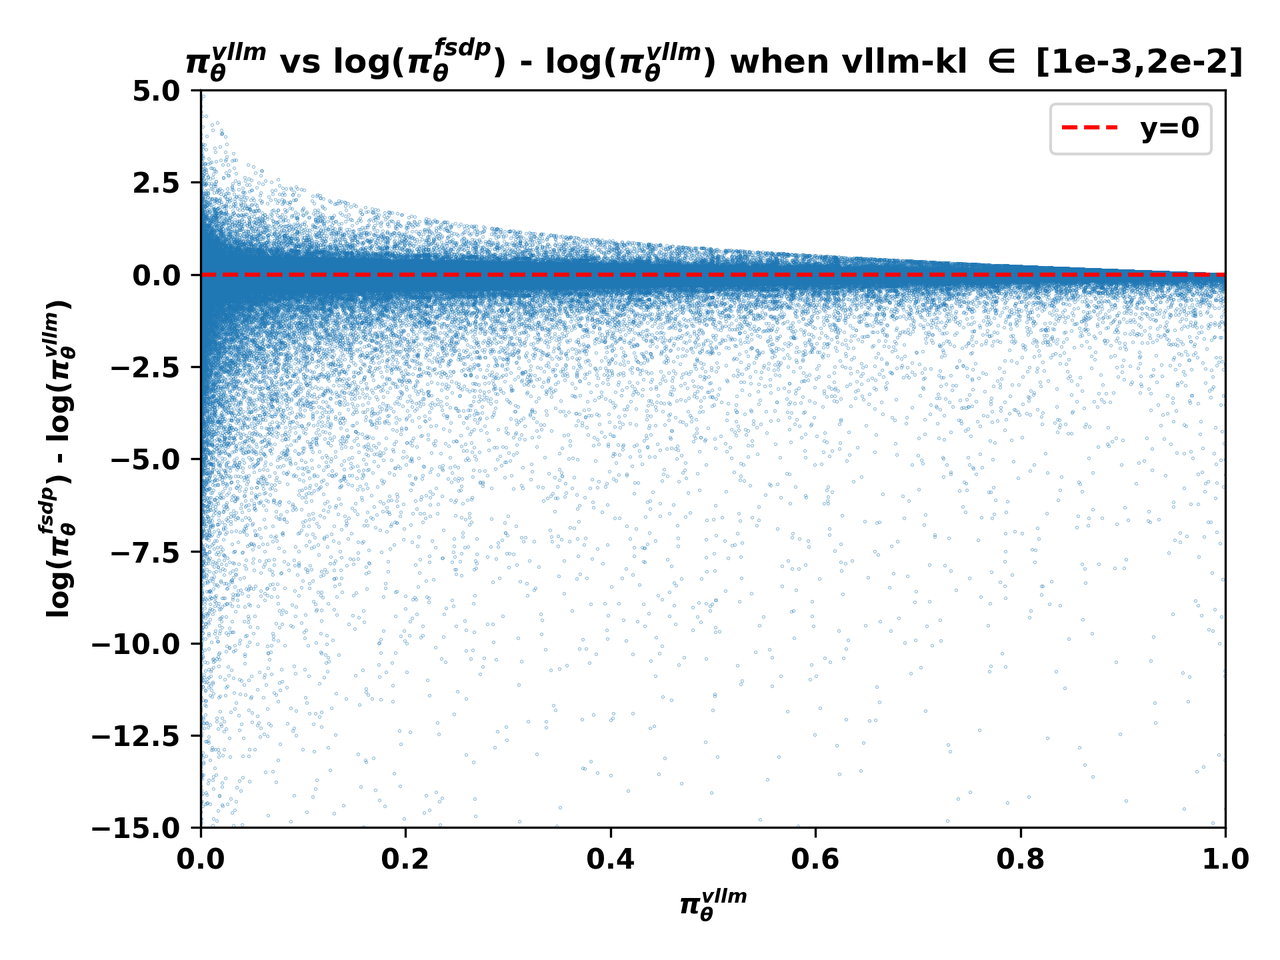
\includegraphics[width=\linewidth,height=0.64\textheight,keepaspectratio]{figures/image-06.png}
\caption*{\textbf{图 4(b)。}第 2 组批次中，词元的 $\piv$ 与 $\log\pif-\log\piv$ 的关系。}
\end{figure}


% source-block: 271211a5-58b7-8092-a67e-f3089c4cf067 (image; source-index: 86)

\begin{figure}[H]
\centering
% source-block: 271211a5-58b7-8092-a67e-f3089c4cf067 (image)
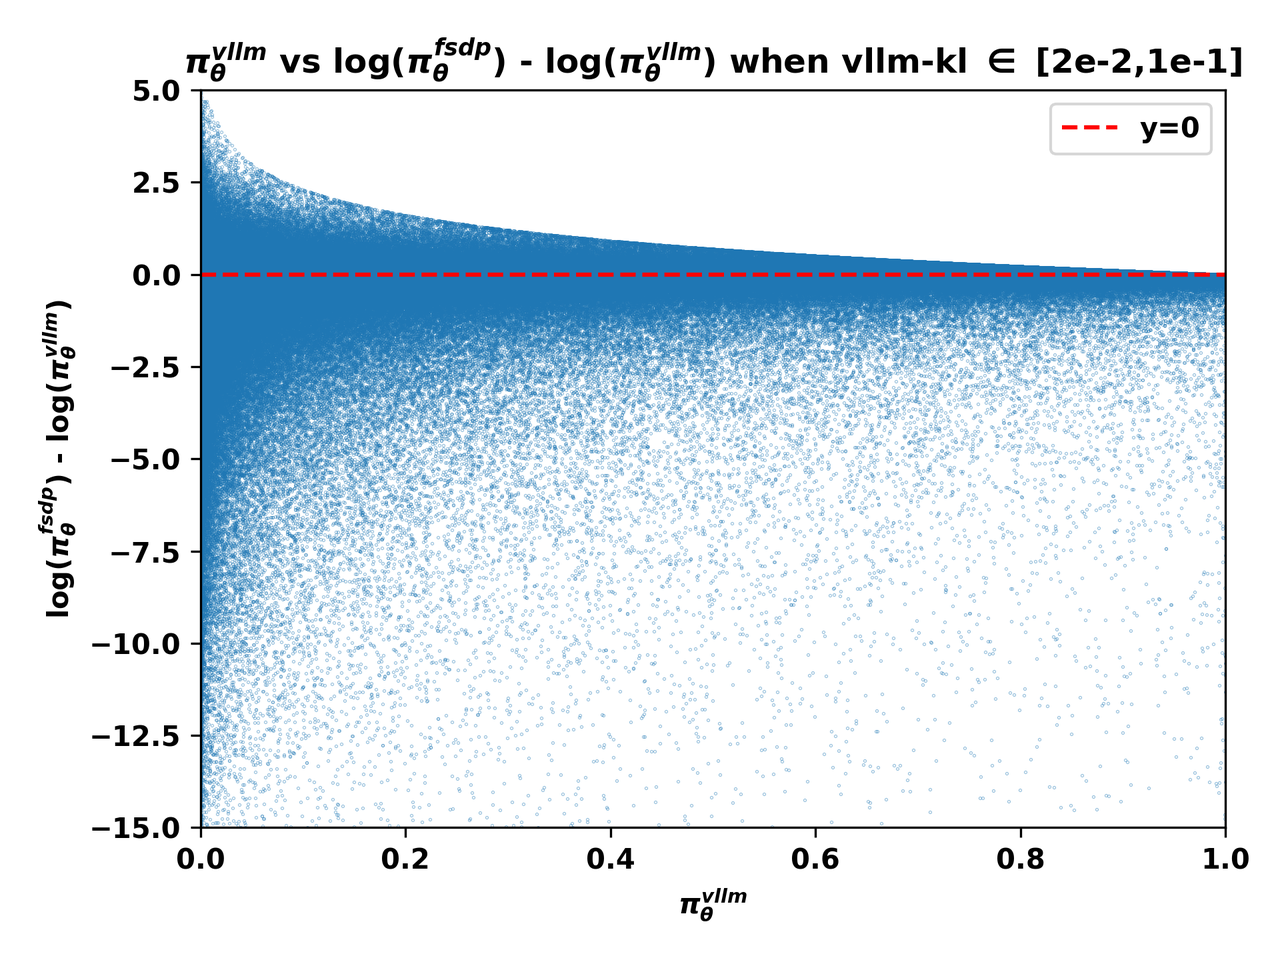
\includegraphics[width=\linewidth,height=0.64\textheight,keepaspectratio]{figures/image-07.png}
\caption*{\textbf{图 4(c)。}第 3 组批次中，词元的 $\piv$ 与 $\log\pif-\log\piv$ 的关系。}
\end{figure}


% source-block: 271211a5-58b7-805f-bcbf-d246ba54362d (text; source-index: 87)

从以上三幅图中，可以清楚观察到：


% source-block: 271211a5-58b7-800a-88b0-cb2ff65c7b6d (numbered_list; source-index: 88)

\begin{enumerate}

\item 当 vLLM 概率 $\piv$ 趋近于零时，不匹配通常更加明显，$\log\pif-\log\piv$ 也更容易出现极端值。

% source-block: 271211a5-58b7-80a8-8b79-d87b04cf6f3c (numbered_list; source-index: 89)

\item L20 GPU 上收集的批次，即第 2、3 组，其训练与推理不匹配主要表现为 FSDP 概率 $\pif$ 显著小于 vLLM 概率 $\piv$。

\end{enumerate}

% source-block: 277211a5-58b7-80bc-ae1a-df54182c0628 (divider; source-index: 90)

% source-block: 271211a5-58b7-8050-b3b1-dbbad2a1eb40 (sub_header; source-index: 91)

\hypertarget{src-271211a5-58b7-8050-b3b1-dbbad2a1eb40}{}
\subsection*{3.4 分布外工具响应放大不匹配}
\phantomsection
\addcontentsline{toc}{subsection}{3.4 分布外工具响应放大不匹配}


% source-block: 277211a5-58b7-80d0-9d87-e202276dc7f9 (sub_sub_header; source-index: 92)

\hypertarget{src-277211a5-58b7-80d0-9d87-e202276dc7f9}{}
\subsubsection*{3.4.1 非首轮输出中的不匹配更严重}


% source-block: 271211a5-58b7-8079-8ad0-d72e0e85ce0b (text; source-index: 93)

第 3 节的发现解释了为什么多轮 TIR 实验中的问题如此突出，尤其是在模型的非首轮输出中。具体过程如下：


% source-block: 271211a5-58b7-809e-8568-f3c1bf646337 (numbered_list; source-index: 94)

\begin{enumerate}

\item 智能体收到工具响应，通常是结构化文本，例如由 \code{<python_output>} 和 \code{</python_output>} 标签包裹的上下文。与预训练和 SFT 数据相比，这类文本属于分布外（OOD）输入。

% source-block: 271211a5-58b7-80a2-82b3-da8b60bb1fdf (numbered_list; source-index: 95)

\item 面对不熟悉的分布外上下文，智能体策略的不确定性增加，因此在后续轮次中更容易采样低概率词元；\href{https://github.com/ltzheng/SimpleTIR}{SimpleTIR} 也观察到了这一现象。

% source-block: 271211a5-58b7-80e1-905f-e8e323252c50 (numbered_list; source-index: 96)

\item 如前所述，低概率词元正是严重不匹配的主要发生位置，因此会为 \code{fsdp-ppl} 和梯度爆炸创造条件。

\end{enumerate}

% source-block: 271211a5-58b7-807f-8974-ccd834bcb702 (text; source-index: 97)

接下来，我们可视化了三组批次中的不匹配情况，每组约 5000 条轨迹，重点比较模型首轮输出与非首轮输出的差异。我们使用两种可视化方式：


% source-block: 271211a5-58b7-8090-a724-cd2cf4996307 (numbered_list; source-index: 98)

\begin{enumerate}

\item \textbf{对数困惑度散点图：}横轴为 vLLM 策略 $\piv$ 计算的困惑度的对数，记作 \code{vllm-log-ppl}；纵轴为 FSDP 策略 $\pif$ 计算的困惑度的对数，记作 \code{fsdp-log-ppl}。

% source-block: 271211a5-58b7-80f8-a083-d8dd1fc23b4c (numbered_list; source-index: 99)

\item \textbf{概率散点图：}横轴为 vLLM 策略 $\piv$ 的词元概率，纵轴为 FSDP 策略 $\pif$ 的词元概率。

\end{enumerate}

% source-block: 271211a5-58b7-80da-a68a-cf9a7e67be87 (text; source-index: 100)

下面给出三组不匹配情况的可视化结果。


% source-block: 271211a5-58b7-802e-8f1c-fa8e9902f933 (bulleted_list; source-index: 101)

\begin{itemize}

\item \textbf{第 1 组：}\code{vllm-kl} $\le10^{-3}$ 的批次。

\end{itemize}

% source-block: 271211a5-58b7-805e-af00-de25affd1d4a (image; source-index: 102)

\begin{figure}[H]
\centering
% source-block: 271211a5-58b7-805e-af00-de25affd1d4a (image)
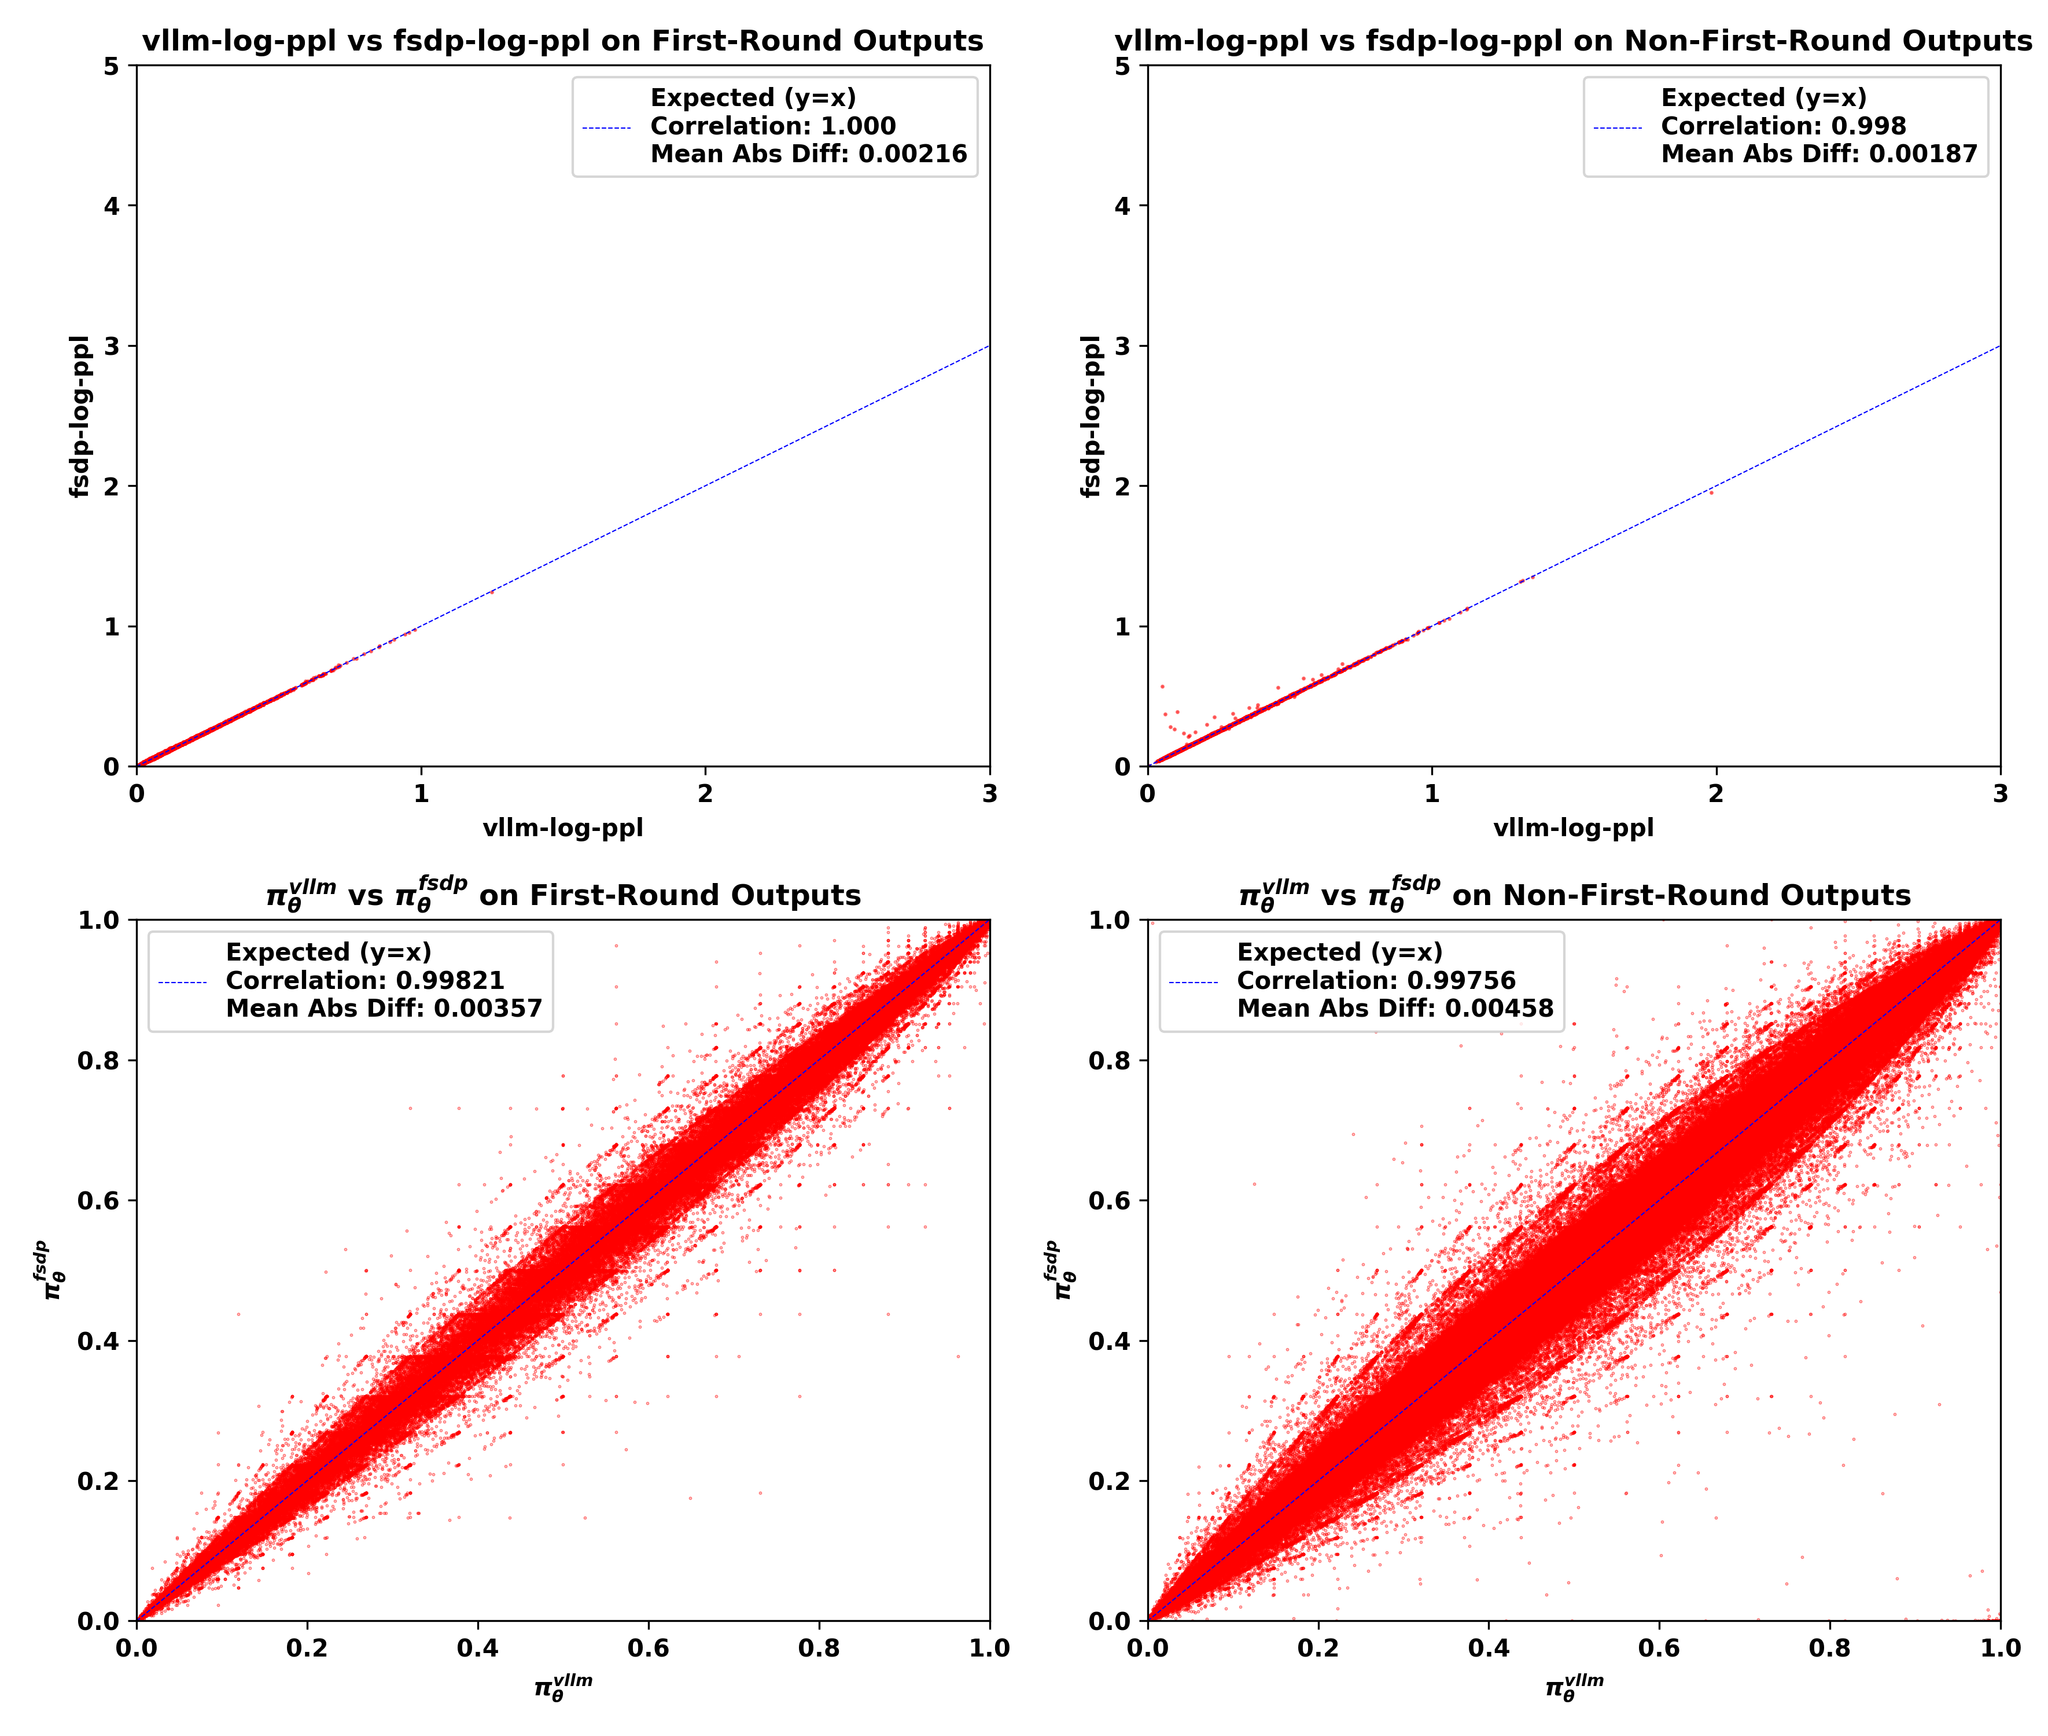
\includegraphics[width=\linewidth,height=0.64\textheight,keepaspectratio]{figures/image-08.png}
\caption*{第 1 组首轮与非首轮输出的不匹配可视化（原文未编号）：\code{vllm-kl} $\le10^{-3}$。}
\end{figure}


% source-block: 271211a5-58b7-804e-84f9-ca41fc298777 (bulleted_list; source-index: 103)

\begin{itemize}

\item \textbf{第 2 组：}\code{vllm-kl} $\in[10^{-3},2\times10^{-2}]$ 的批次。

\end{itemize}

% source-block: 271211a5-58b7-80cb-8597-da22a85d90da (image; source-index: 104)

\begin{figure}[H]
\centering
% source-block: 271211a5-58b7-80cb-8597-da22a85d90da (image)
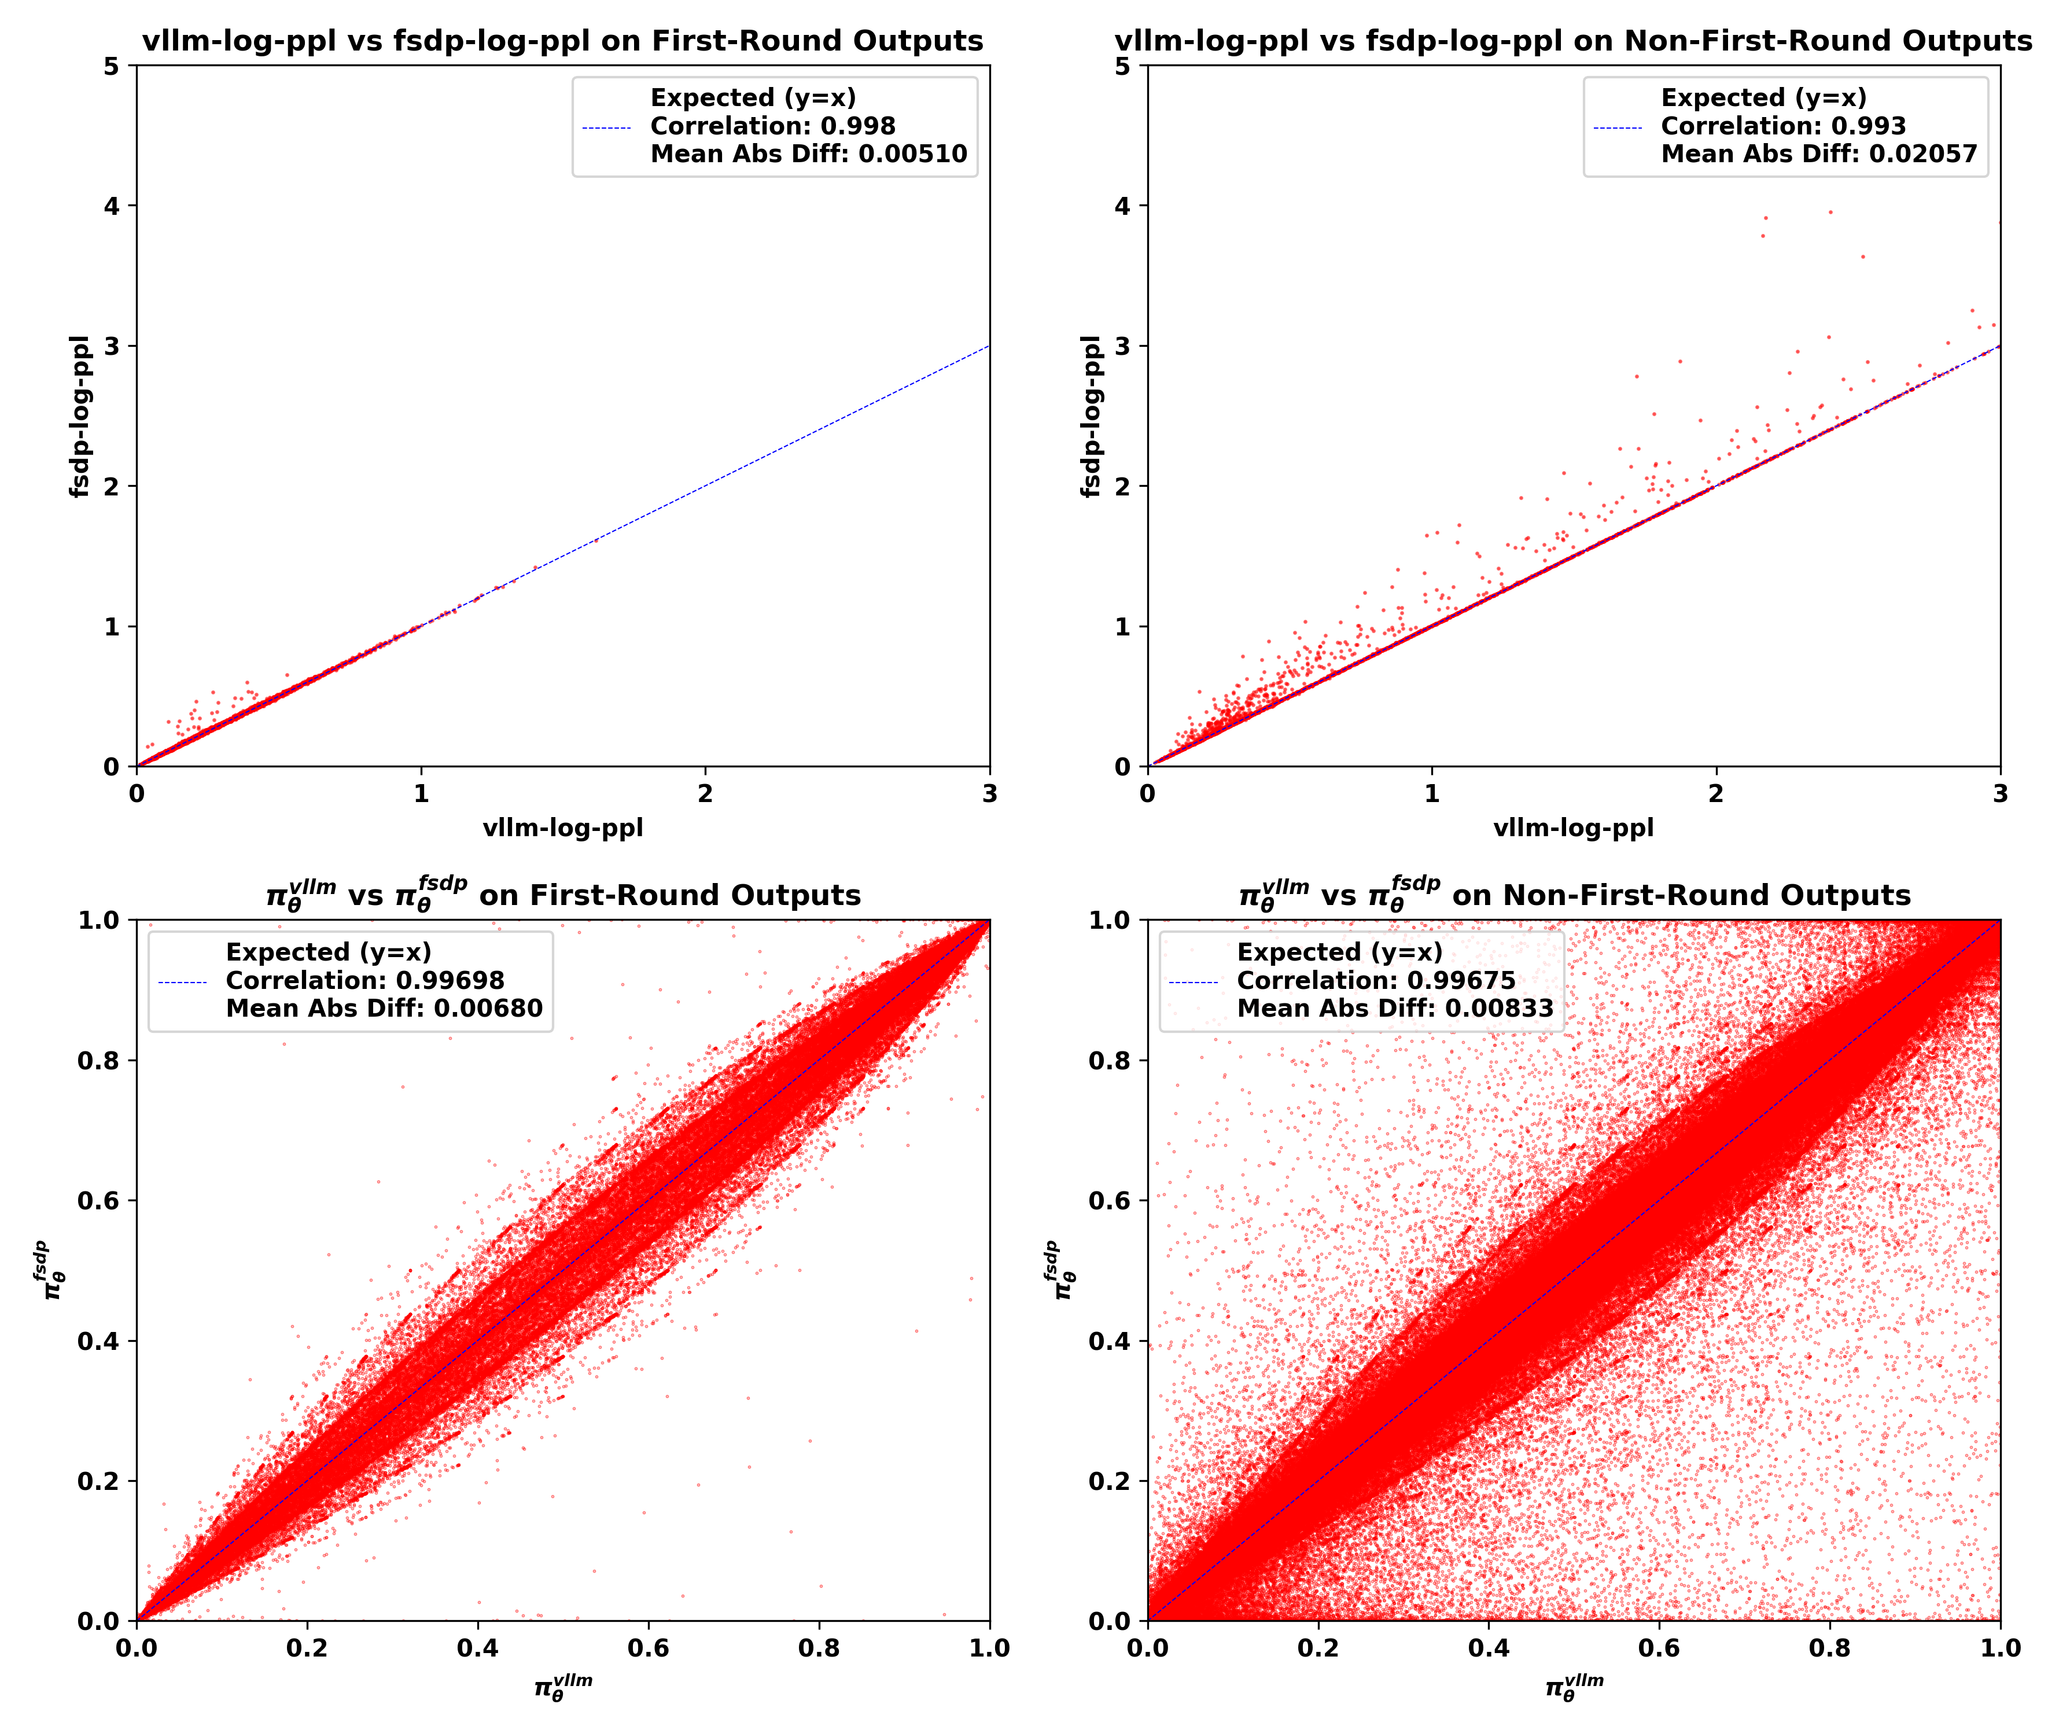
\includegraphics[width=\linewidth,height=0.64\textheight,keepaspectratio]{figures/image-09.png}
\caption*{第 2 组首轮与非首轮输出的不匹配可视化（原文未编号）：\code{vllm-kl} $\in[10^{-3},2\times10^{-2}]$。}
\end{figure}


% source-block: 271211a5-58b7-807c-b2f5-db46f3b9cf4a (bulleted_list; source-index: 105)

\begin{itemize}

\item \textbf{第 3 组：}\code{vllm-kl} $\in[2\times10^{-2},10^{-1}]$ 的批次。

\end{itemize}

% source-block: 271211a5-58b7-8024-8265-c6f33580b3be (image; source-index: 106)

\begin{figure}[H]
\centering
% source-block: 271211a5-58b7-8024-8265-c6f33580b3be (image)
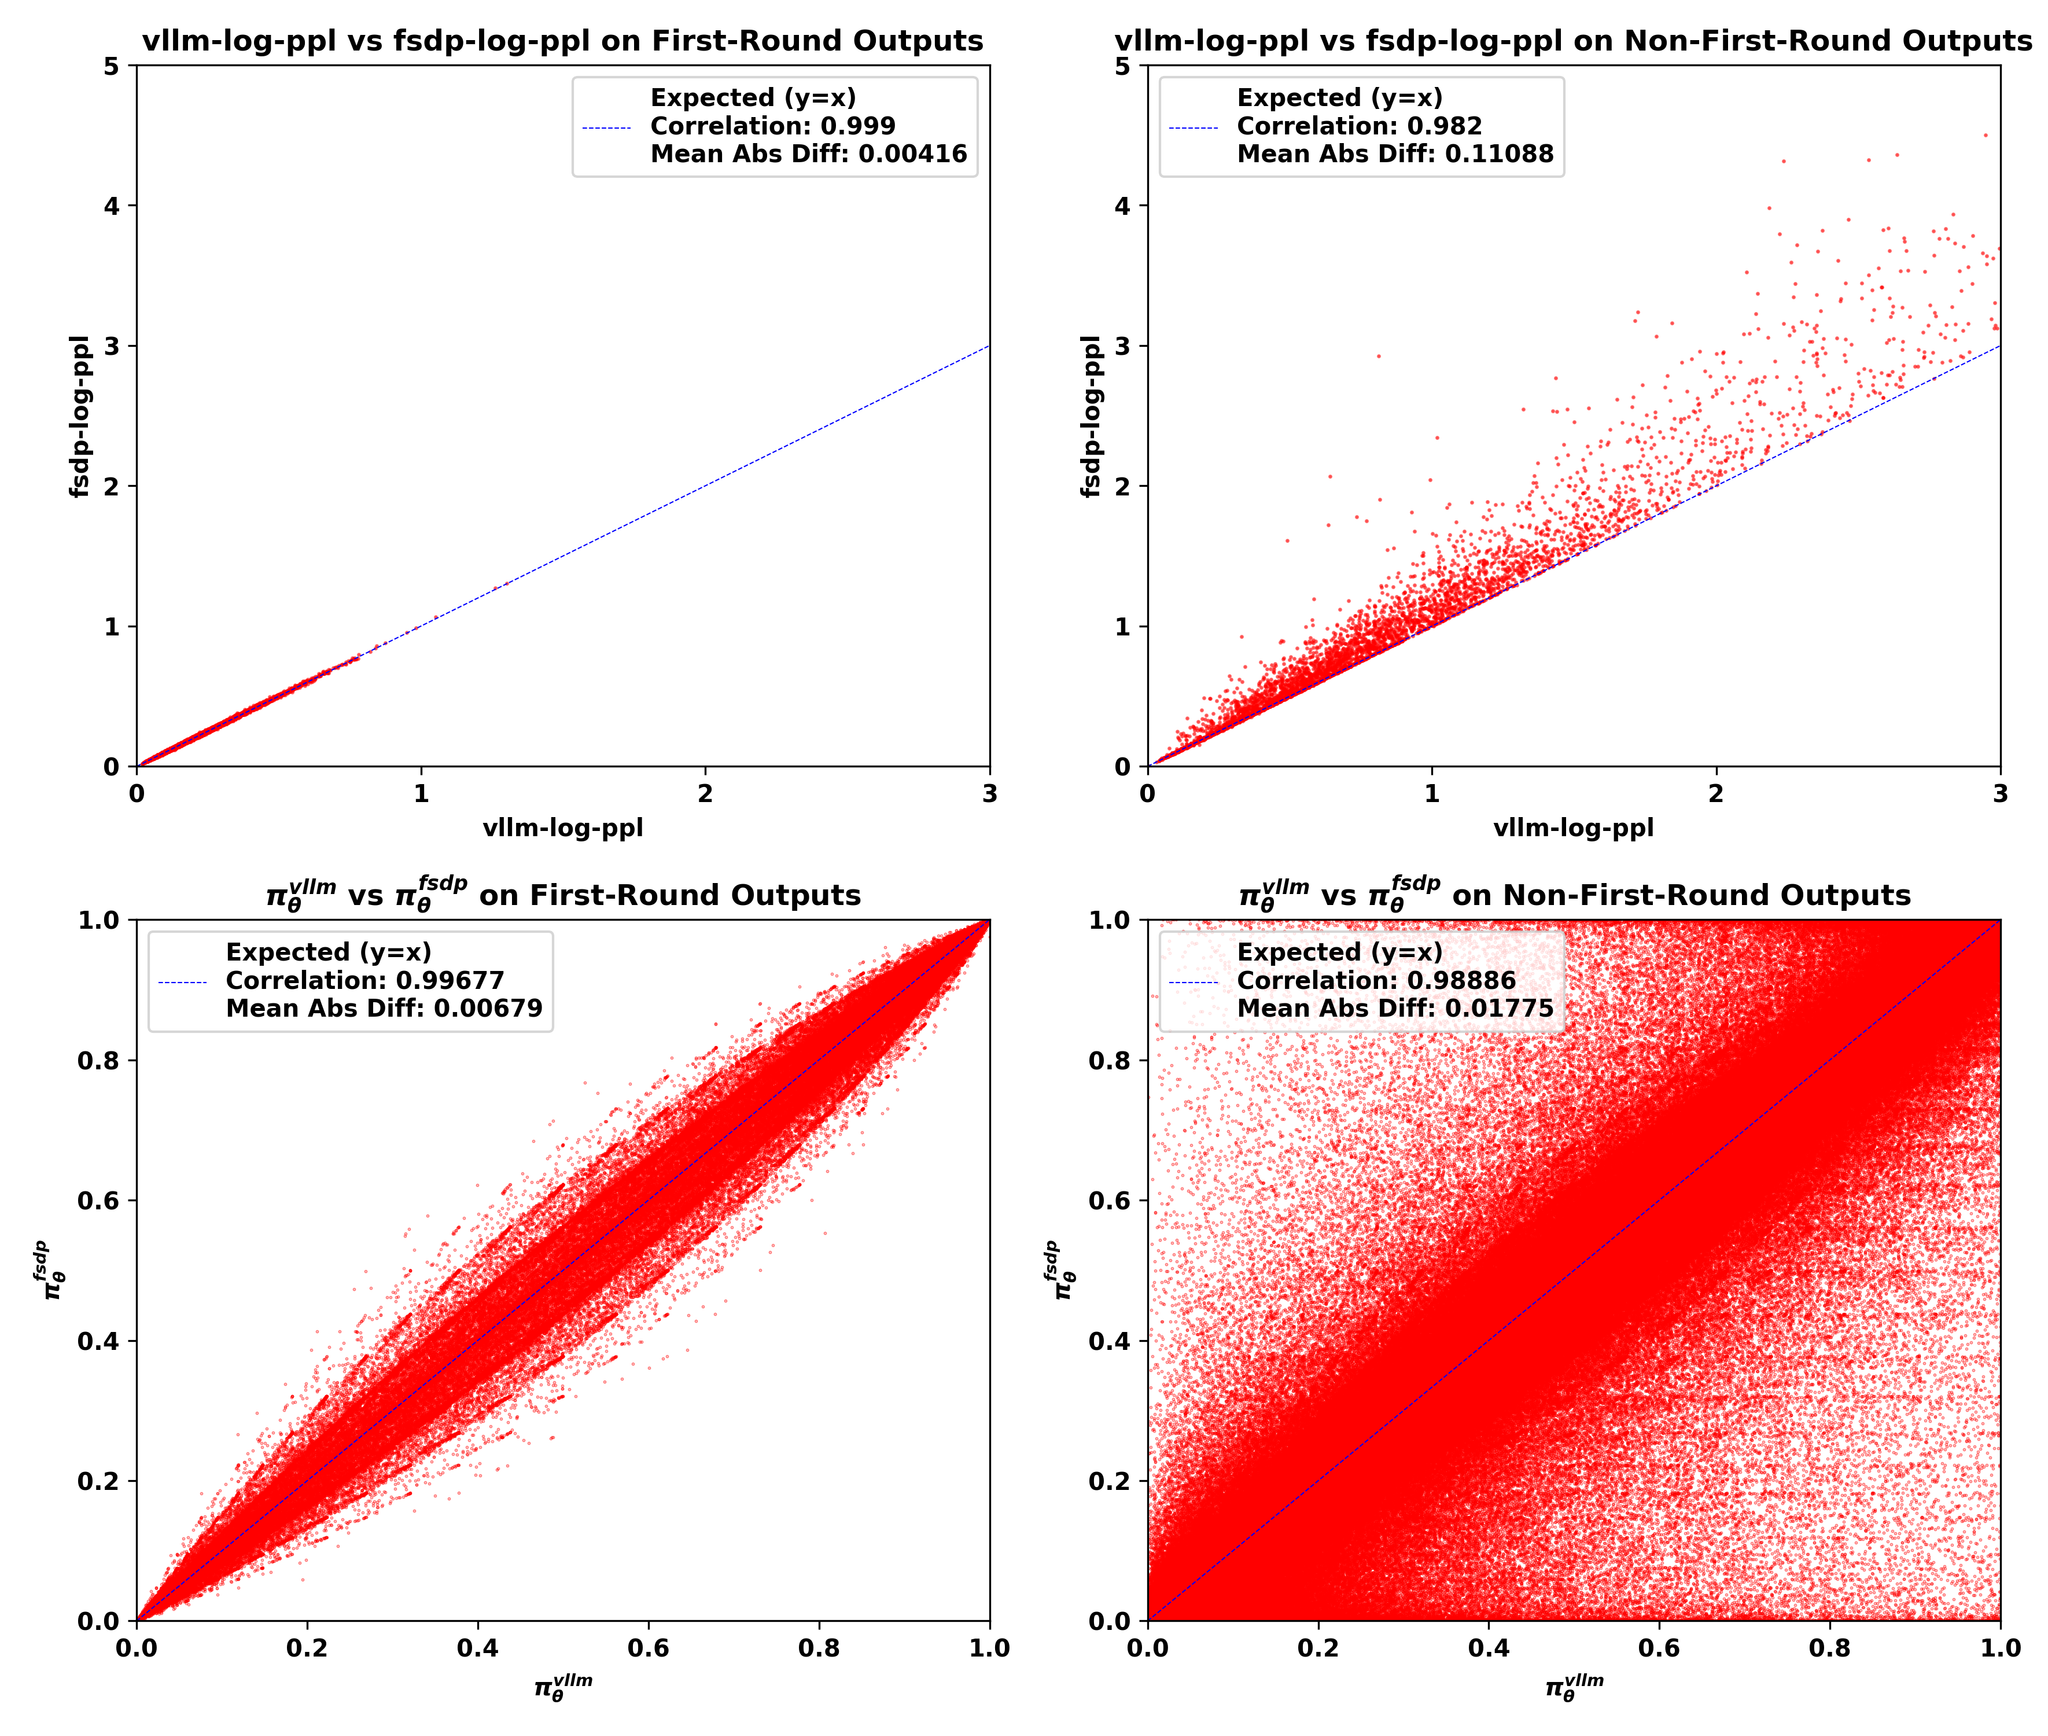
\includegraphics[width=\linewidth,height=0.64\textheight,keepaspectratio]{figures/image-10.png}
\caption*{第 3 组首轮与非首轮输出的不匹配可视化（原文未编号）：\code{vllm-kl} $\in[2\times10^{-2},10^{-1}]$。}
\end{figure}


% source-block: 271211a5-58b7-80e8-bb59-d8c2c4839f75 (text; source-index: 107)

从可视化结果可以观察到：


% source-block: 271211a5-58b7-80d4-bd8f-c072e9833bd0 (numbered_list; source-index: 108)

\begin{enumerate}

\item 非首轮输出的 \code{vllm-log-ppl} 通常大于首轮输出，说明模型面对不熟悉的分布外上下文时，会采样更多低概率词元。

% source-block: 271211a5-58b7-80da-9a4f-f339c3272a45 (numbered_list; source-index: 109)

\item 不匹配主要发生在非首轮输出中：与首轮输出相比，FSDP 与 vLLM 策略之间在对数困惑度和词元概率上的平均绝对差都更大，皮尔逊相关系数也更低。

% source-block: 271211a5-58b7-80b7-9b90-e3adee7c73c7 (numbered_list; source-index: 110)

\item 随着 \code{vllm-kl} 增大，训练与推理不匹配的恶化主要发生在非首轮输出。

% source-block: 271211a5-58b7-80ed-83ee-dd914cdf139e (numbered_list; source-index: 111)

\item 不匹配始终表现为 \code{fsdp-log-ppl} 大于 \code{vllm-log-ppl}，表明 FSDP 引擎产生了更极端的低概率词元。

\end{enumerate}

% source-block: 277211a5-58b7-80b6-9438-f97089a3b349 (divider; source-index: 112)

% source-block: 277211a5-58b7-805b-b021-d722c4d2eb3c (sub_sub_header; source-index: 113)

\hypertarget{src-277211a5-58b7-805b-b021-d722c4d2eb3c}{}
\subsubsection*{3.4.2 工具调用越多，训练越不稳定}


% source-block: 277211a5-58b7-803e-a52c-f2b1fd47d9f1 (text; source-index: 114)

下面的实验也表明，分布外工具响应会加剧训练与推理不匹配及训练不稳定性。我们在 H20 GPU 上，以 Qwen3-14B-Base 为基础模型开展异策略 GRPO 实验，设置 \code{clip higher=0.28}，并使用 4 个小批次。单条轨迹中工具调用次数的上限，即超参数 \code{max_tool_turn}，分别设为 20 和 100。图 5 和图 6 展示了结果：随着工具调用次数增多，训练更早崩溃；崩溃时，各次实验均观察到了梯度爆炸与 \code{vllm-kl} 爆炸。


% source-block: 277211a5-58b7-80fc-844d-edb200c466dc (image; source-index: 115)

\begin{figure}[H]
\centering
% source-block: 277211a5-58b7-80fc-844d-edb200c466dc (image)
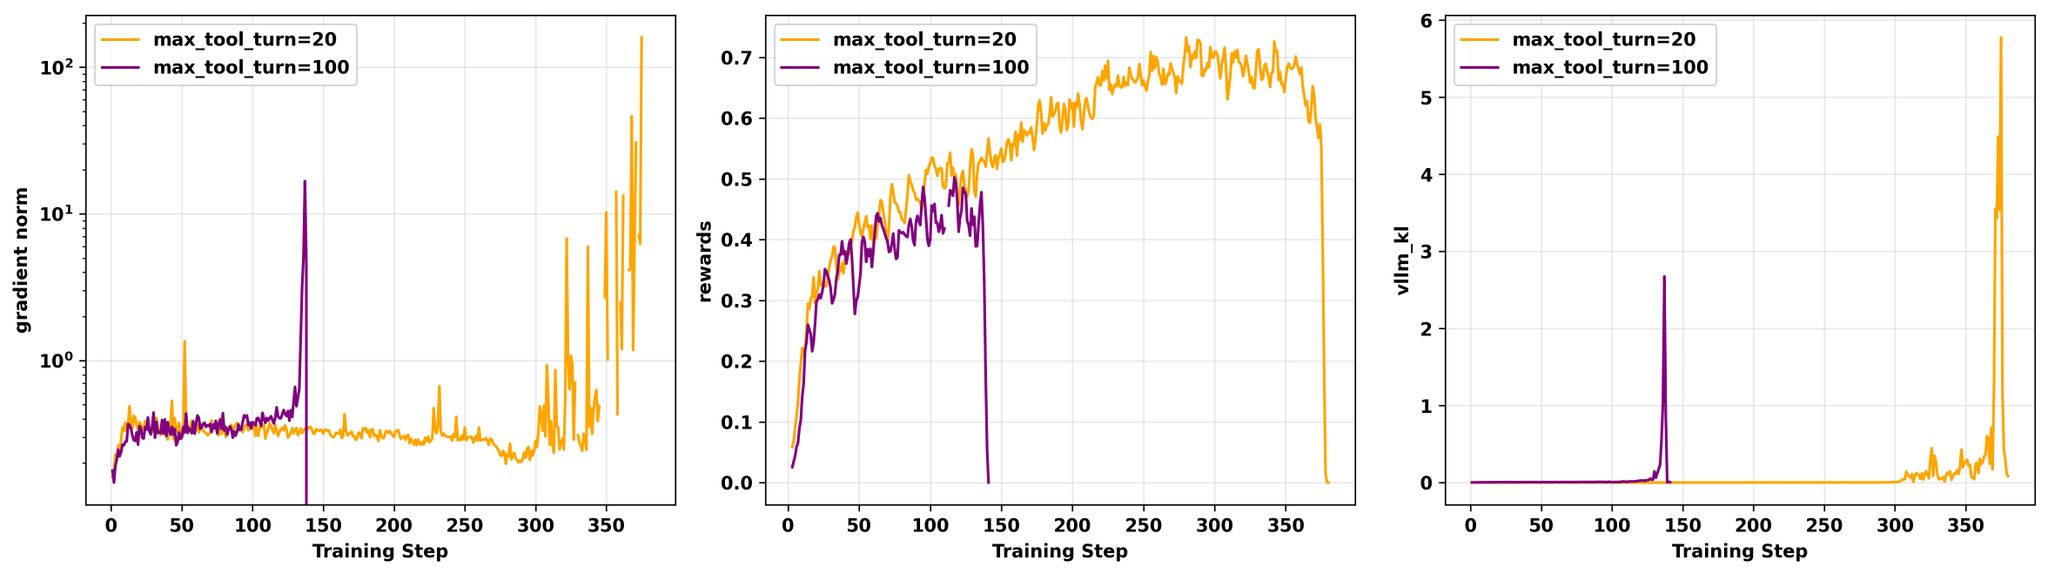
\includegraphics[width=\linewidth,height=0.64\textheight,keepaspectratio]{figures/image-11.jpg}
\caption*{\textbf{图 5。}不同 \code{max_tool_turn} 设置下，异策略 GRPO 的梯度范数（左）、奖励（中）与 \code{vllm-kl}（右）。均在 H20 上，以 Qwen3-14B-Base 为基础模型，设置 \code{clip higher=0.28}，使用 4 个小批次。}
\end{figure}


% source-block: 277211a5-58b7-80ed-902c-f6a8bd68c885 (image; source-index: 116)

\begin{figure}[H]
\centering
% source-block: 277211a5-58b7-80ed-902c-f6a8bd68c885 (image)
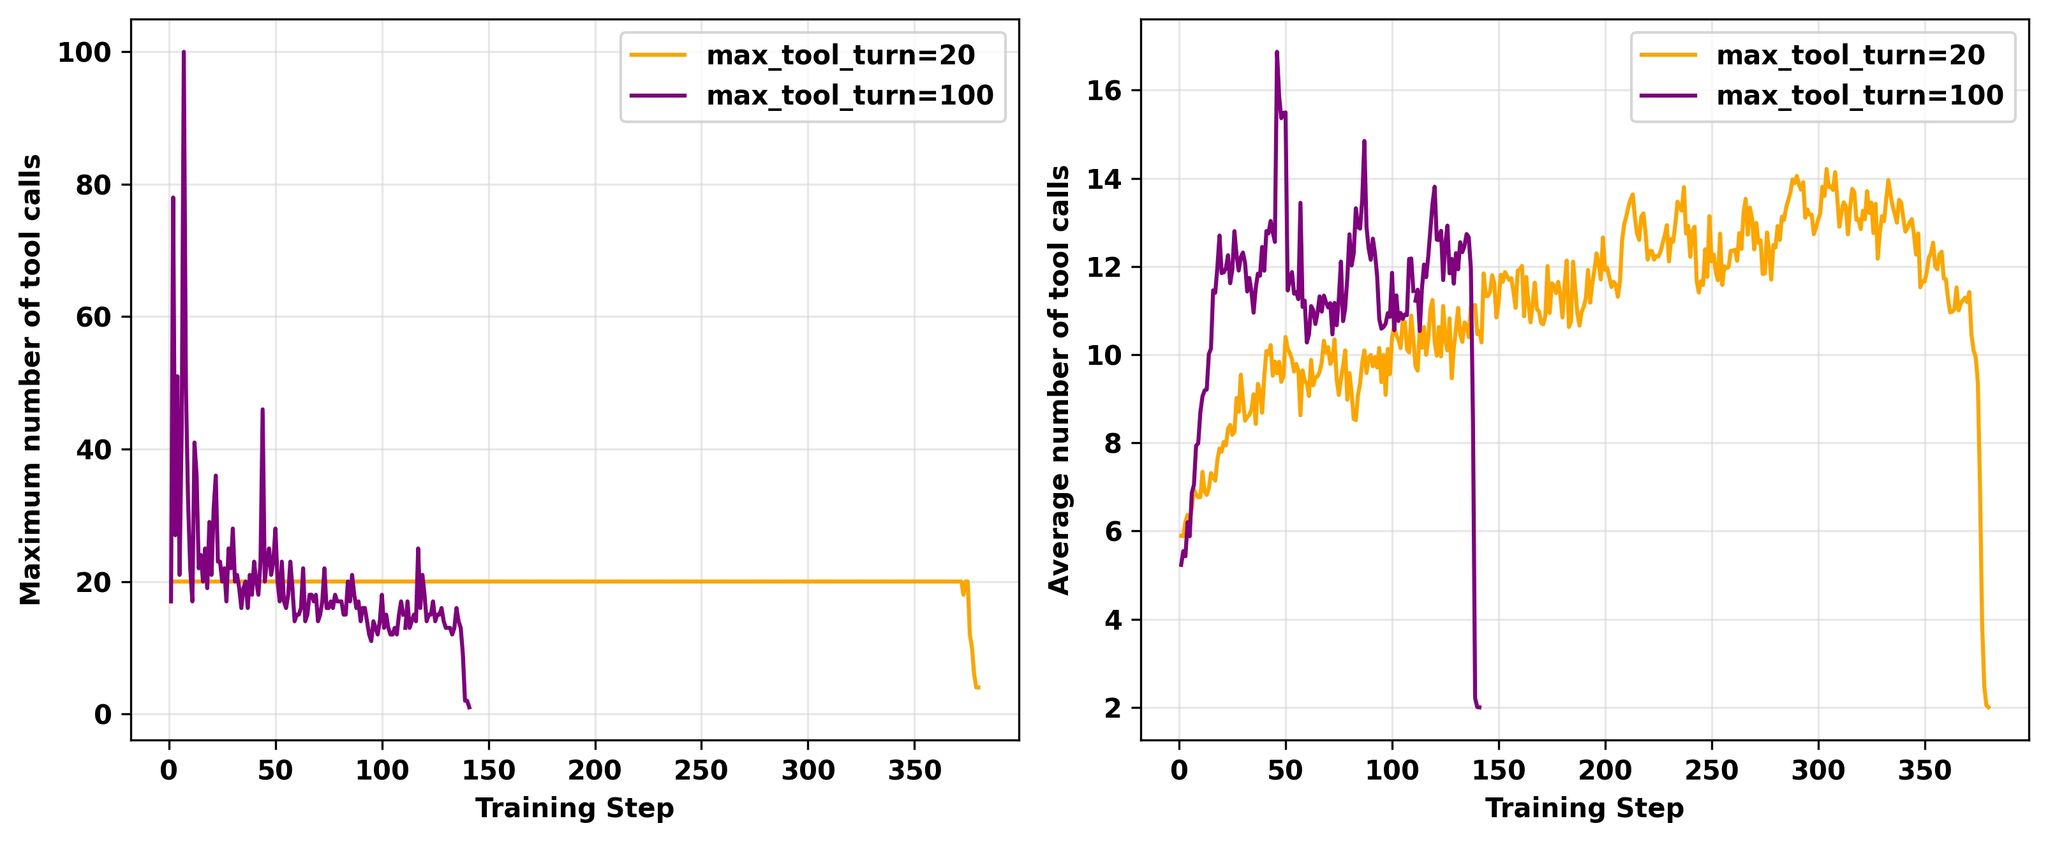
\includegraphics[width=\linewidth,height=0.64\textheight,keepaspectratio]{figures/image-12.jpg}
\caption*{\textbf{图 6。}不同 \code{max_tool_turn} 设置下，异策略 GRPO 的最大工具调用次数（左）与平均工具调用次数（右）。均在 H20 上，以 Qwen3-14B-Base 为基础模型，设置 \code{clip higher=0.28}，使用 4 个小批次。}
\end{figure}


% source-block: 277211a5-58b7-8084-89d4-ea00c3bdbc3b (divider; source-index: 117)

% source-block: 271211a5-58b7-80c9-ad90-f8aa1353bfe1 (sub_header; source-index: 118)

\hypertarget{src-271211a5-58b7-80c9-ad90-f8aa1353bfe1}{}
\subsection*{3.5 环境因素：硬件的关键作用}
\phantomsection
\addcontentsline{toc}{subsection}{3.5 环境因素：硬件的关键作用}


% source-block: 271211a5-58b7-8008-a5ba-ec1353923d67 (text; source-index: 119)

最后，我们发现物理硬件是一个关键变量。\textbf{完全相同的代码与模型，在不同 GPU 硬件上产生的不匹配程度差异巨大。}为评估硬件差异，我们在相同代码环境与超参数下运行同策略算法，只更换用于推理和训练的 GPU。图 7 分别展示了 L20、H20 和 A100 上的训练动态。


% source-block: 271211a5-58b7-807d-b017-dc3d1d908ff8 (image; source-index: 120)

\begin{figure}[H]
\centering
% source-block: 271211a5-58b7-807d-b017-dc3d1d908ff8 (image)
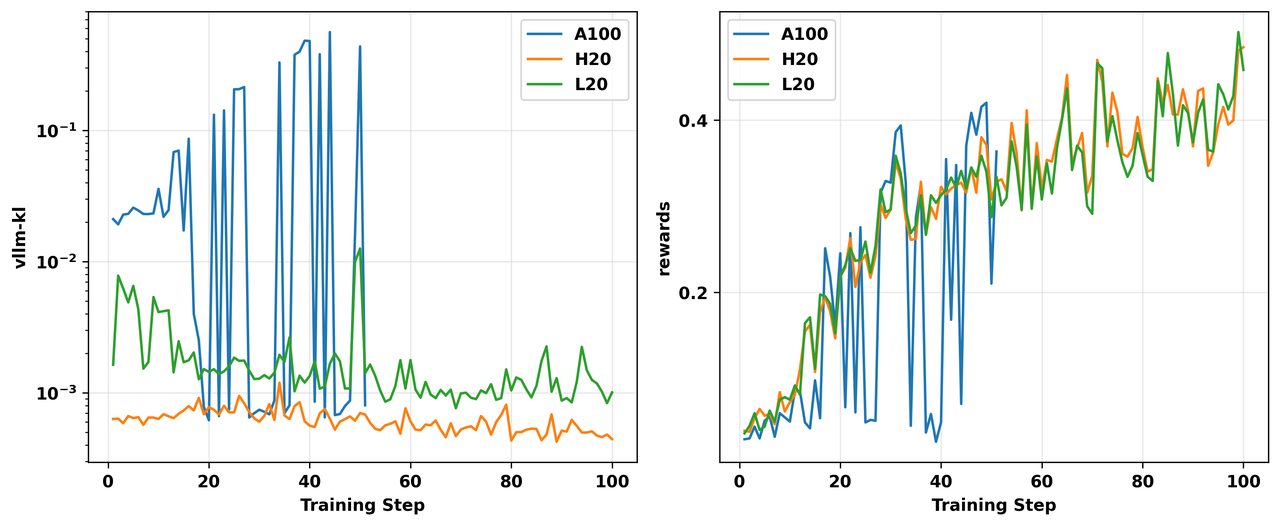
\includegraphics[width=\linewidth,height=0.64\textheight,keepaspectratio]{figures/image-13.png}
\caption*{\textbf{图 7。}不同 GPU 上，同策略 GRPO 实验的 \code{vllm-kl}（左）与奖励（右）。所有实验均使用相同代码与环境。}
\end{figure}


% source-block: 271211a5-58b7-8016-87f5-c640d0f8d5f0 (text; source-index: 121)

在我们的实验中，\code{vllm-kl} 的量级基本满足 \textbf{H20 $<$ L20 $<$ A100}。具体而言，H20 通常为 $5\times10^{-4}$ 至 $10^{-3}$，L20 约为 $10^{-3}$ 至 $10^{-2}$，A100 则主要处于 $10^{-2}$ 至 $1$。A100 上严重的训练与推理不匹配使正常训练难以进行，奖励曲线高度不稳定。


% source-block: 2a8211a5-58b7-8062-8a6a-ed98d6c13b5f (text; source-index: 122)

我们发现，在 A100 GPU 实验中，关闭 vLLM 的级联注意力（cascade attention）尤其有助于减小不匹配。相关结果见第 4.2.4 节。


% source-block: 271211a5-58b7-8077-a02a-f7bad00d87a1 (text; source-index: 123)

最有说服力的证据来自一次恢复实验：我们将 L20 上失败实验的检查点转移到 H20 GPU 上继续训练（见图 8），训练立即稳定并恢复，说明硬件对该问题具有直接且显著的影响。


% source-block: 271211a5-58b7-8039-b3b1-ddc62d10f463 (image; source-index: 124)

\begin{figure}[H]
\centering
% source-block: 271211a5-58b7-8039-b3b1-ddc62d10f463 (image)
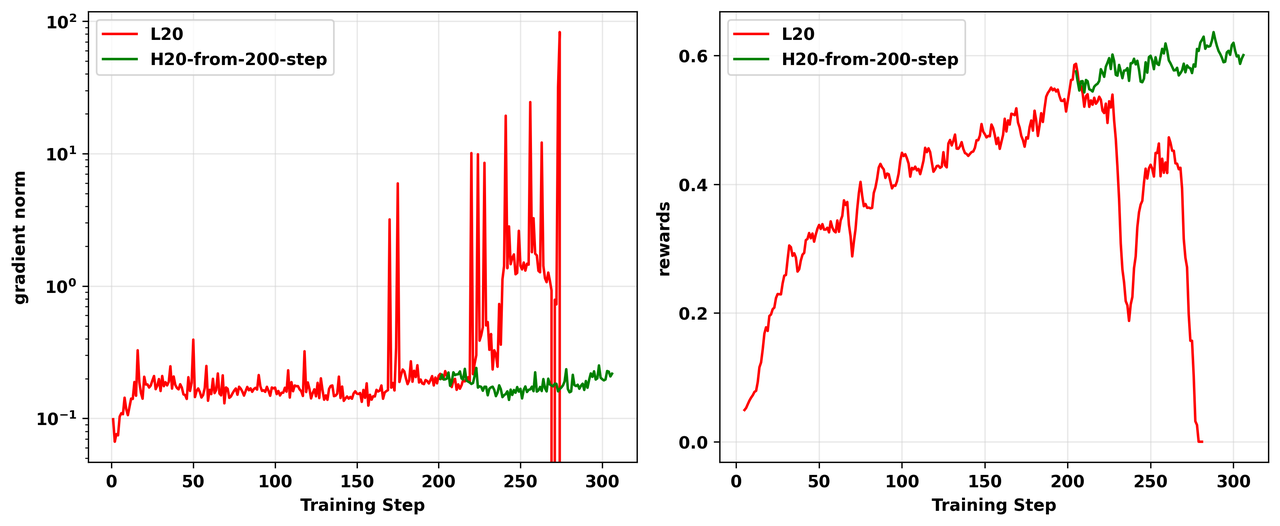
\includegraphics[width=\linewidth,height=0.64\textheight,keepaspectratio]{figures/image-14.png}
\caption*{\textbf{图 8。}L20 与 H20 上同策略 GRPO 实验的梯度范数（左）和奖励（右）。H20 实验（绿线）从失败 L20 实验（红线）的第 200 步检查点启动。}
\end{figure}


% source-block: 277211a5-58b7-8060-a17d-d48fb6c48d1e (divider; source-index: 125)

% source-block: 271211a5-58b7-8029-a918-f29c6ca7198d (sub_header; source-index: 126)

\hypertarget{src-271211a5-58b7-8029-a918-f29c6ca7198d}{}
\subsection*{3.6 不匹配并非静态：由优化驱动的恶性循环}
\phantomsection
\addcontentsline{toc}{subsection}{3.6 不匹配并非静态：由优化驱动的恶性循环}


% source-block: 271211a5-58b7-802e-a9bf-ea88ac4a7010 (text; source-index: 127)

人们可能以为，训练与推理不匹配是硬件和软件栈的静态属性。但下面的“批次过滤”（batch-filter）实验表明，\textbf{不匹配与训练动态及模型状态相互耦合。}


% source-block: 271211a5-58b7-8087-ab3d-c93b7634665c (text; source-index: 128)

在批次过滤实验中，每个训练步采用如下更新策略：若采集批次的 \code{vllm-kl} 大于阈值，则跳过该批次上的参数更新，因为这类更新容易引发训练崩溃；随后直接进入下一步，继续收集数据，直到取得 \code{vllm-kl} 低于阈值的批次，再更新模型。


% source-block: 271211a5-58b7-80ff-9032-c093eab4840b (text; source-index: 129)

该实验的逻辑是：如果不匹配程度完全独立于模型输出分布和训练动态，那么不同训练步中的 \code{vllm-kl} 应具有相同分布。然而，图 9 表明，一旦模型进入某种状态，就开始持续生成高度不匹配的批次，使训练实际上陷入停滞。再结合其他实验中 \code{vllm-kl} 与 \code{fsdp-ppl} 螺旋式攀升的现象（图 10），这些证据指向一个危险的反馈回路。


% source-block: 271211a5-58b7-80db-ad92-f9d2ded4a453 (image; source-index: 130)

\begin{figure}[H]
\centering
% source-block: 271211a5-58b7-80db-ad92-f9d2ded4a453 (image)
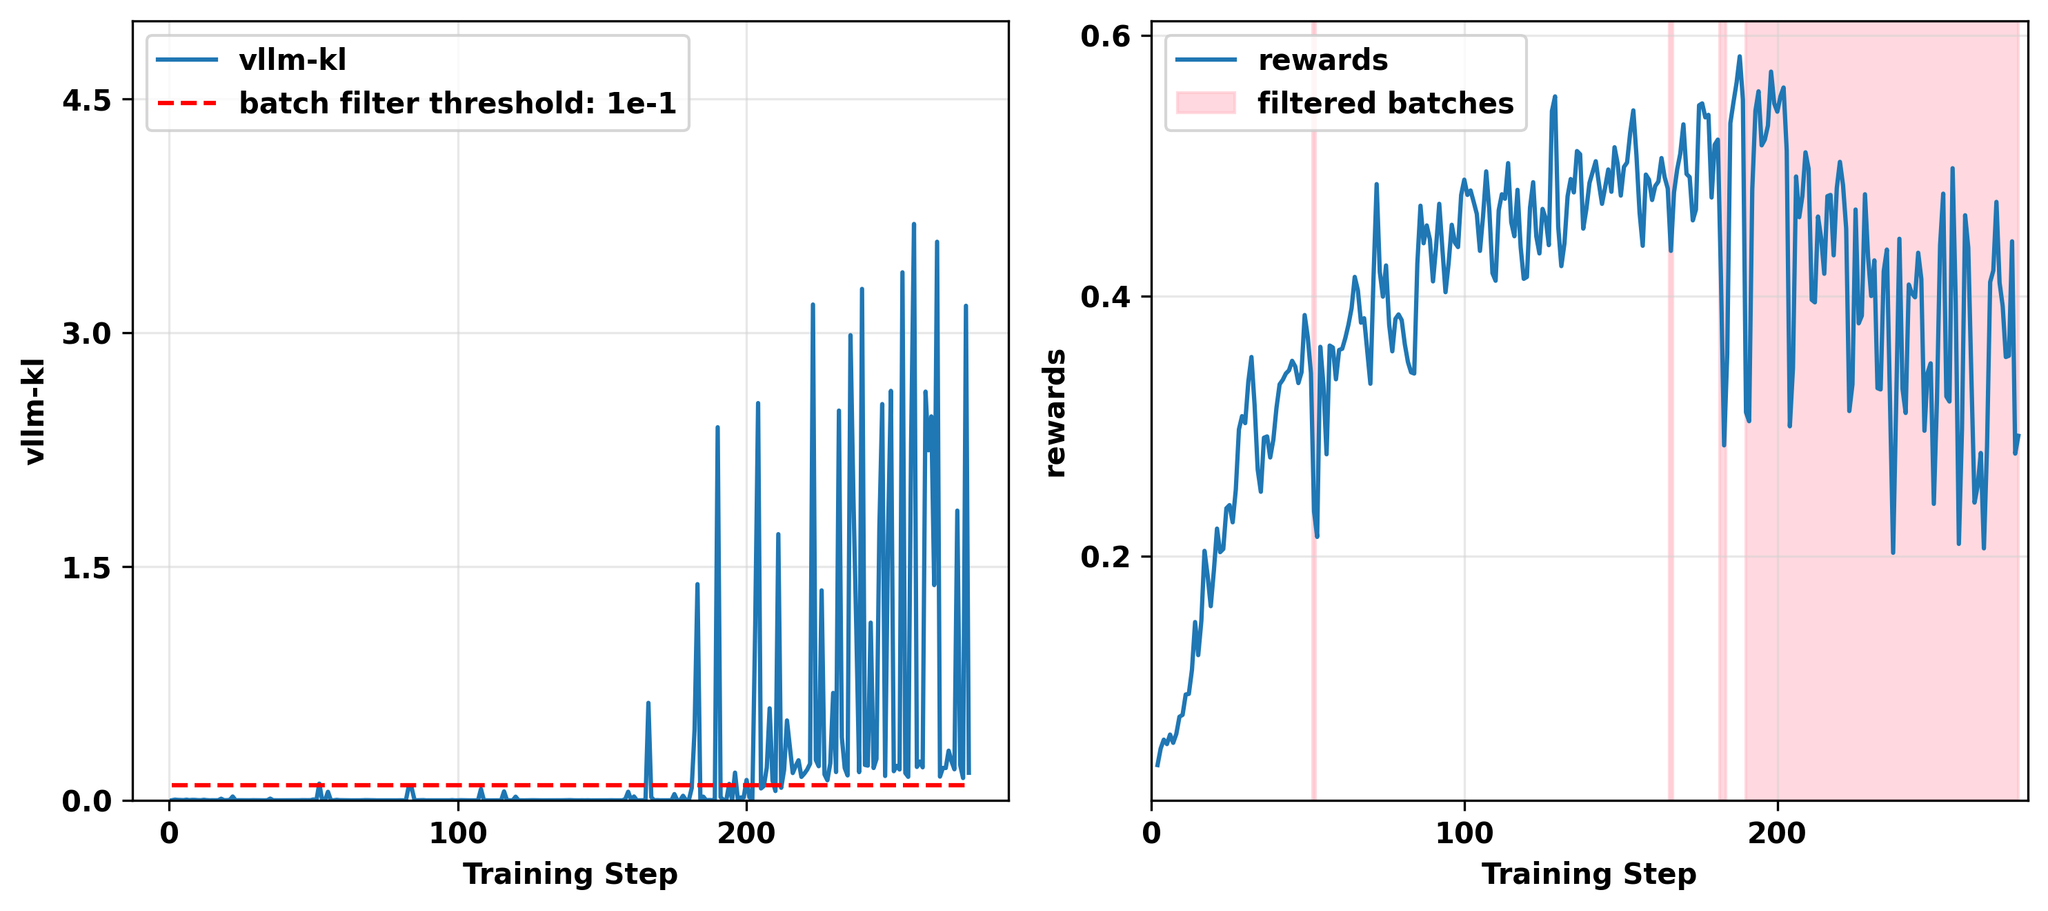
\includegraphics[width=\linewidth,height=0.64\textheight,keepaspectratio]{figures/image-15.png}
\caption*{\textbf{图 9。}同策略“批次过滤”实验的 \code{vllm-kl}（左）与奖励（右）。过滤阈值设为 0.1；批次被过滤的训练步用粉色标出。}
\end{figure}


% source-block: 271211a5-58b7-80eb-8c3c-fc81889860ed (image; source-index: 131)

\begin{figure}[H]
\centering
% source-block: 271211a5-58b7-80eb-8c3c-fc81889860ed (image)
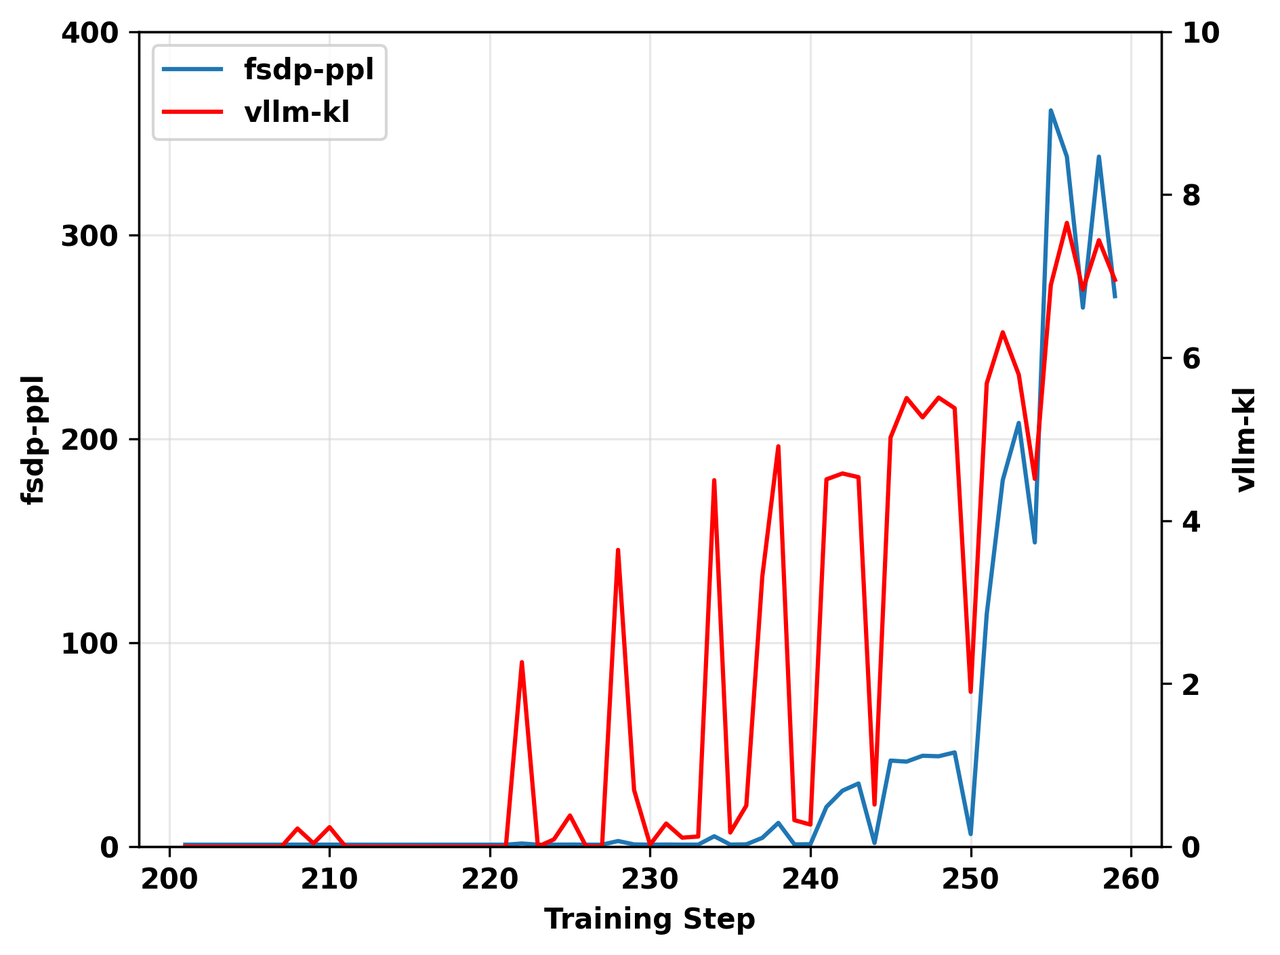
\includegraphics[width=\linewidth,height=0.64\textheight,keepaspectratio]{figures/image-16.png}
\caption*{\textbf{图 10。}一次同策略实验中，\code{vllm-kl} 与 \code{fsdp-ppl} 随训练步数的变化。两条曲线呈现相互关联、螺旋式上升的模式。}
\end{figure}


% source-block: 271211a5-58b7-8003-8533-ec98b0d66201 (text; source-index: 132)

\textbf{我们推测，这是以下两阶段级联失效造成的：}


% source-block: 271211a5-58b7-80ff-81ad-fa6e9105dbf4 (numbered_list; source-index: 133)

\begin{enumerate}

\item \textbf{阶段 1：数值敏感性增加。}强化学习优化器将模型权重推入 \code{bfloat16} 相对精度较低的数值范围，例如非常小或非常大的值。\footnote{译注：此处忠实保留作者的机制假设。对普通正规数，BF16 的相对间隔大致固定；极端值还可能涉及上溢、下溢或次正规数。因此，这段表述不应被当作已由本文实验直接验证的浮点数性质。}

% source-block: 271211a5-58b7-8080-8d52-fb6ef5e4adc4 (numbered_list; source-index: 134)

\item \textbf{阶段 2：内核驱动的误差放大。}这些初始的微小 \code{bfloat16} 量化误差进入 vLLM 与 FSDP 的不同内核实现。不同的计算顺序充当非线性放大器，使很小的初始偏差不断累积，最终造成 logits 的巨大差异。

\end{enumerate}

% source-block: 271211a5-58b7-80d5-a007-e96da4174eb1 (text; source-index: 135)

由此形成恶性反馈回路：不匹配产生有偏且噪声较大的梯度；这些梯度可能进一步将参数推向数值敏感区域；这又加剧下一次迭代的不匹配，直至系统崩溃。


% source-block: 277211a5-58b7-80cc-bdf2-edc86beb5fbc (divider; source-index: 136)
